\section{Java Reflection}

\subsection{Reflection in Java}

\subsubsection{Introduction}

The \textbf{Java Core Reflection API} provides a small, type-safe, and secure API that supports introspection about the classes and objects in the current Java Virtual Machine.

\textbf{If permitted by security policy, the API can be used to}:
\begin{itemize}
	\item construct new class instances and new array
	\item access and modify fields of object and classes
	\item invoke methods on object and classes, and
	\item access and modify elements of array
\end{itemize}

Intercession on classes and objects is forbidden

\subsubsection{Introduction (Cont'd)}

\textbf{The Java application that benefint from introspection are}:

\begin{itemize}
	\item automatic documentation (javac, javadoc, ...)
	\item tools for IDEs: browsers, inspectors, debuggers, ...
	\item serialization / deserialization
	- construction of a binary representation for backup or transmission;
	- re-creating an object based on its serialized form;
	\item RMI
	- serialization of arguments and return values;
	- identification of remote methods.
\end{itemize}

\subsubsection{Classes and Interfaces for Reflection}

\textbf{Since Java < 12}

- java.lang.Object
	- java.lang.Class
	- java.lang.reflect.Member
		- java.lang.reflect.Field (Member)
		- java.lang.reflect.Method (Member)
		- java.lang.reflect.Constructor (Member)

- boolean.class, char.class, int.class, double.class, ...

\textbf{Since Java 13}

- java.lang.Object
	- java.lang.Class
	- java.lang.reflect.Member
	- java.lang.reflect.AccessibleObject
		- java.lang.reflect.Field (Member)
		- java.lang.reflect.Method (Member)
		- java.lang.reflect.Constructor (Member)
	- java.lang.reflect.Proxy
	- java.lang.reflect.InvocationHandler

- boolean.class, char.class, int.class, double.class, ...

\textbf{Since Java 15}

- java.lang.Object
	- java.lang.Class
	- java.lang.reflect.Member
	- java.lang.reflect.AccessibleObject
		- java.lang.reflect.Field (Member)
		- java.lang.reflect.Method (Member)
		- java.lang.reflect.Constructor (Member)
	- java.lang.reflect.Proxy
	- java.lang.reflect.InvocationHandler
	- java.lang.annotation.Annotation
	- java.lang.instrument.Instrumentation

boolean.class, char.class, int.class, double.class, ...

\subsubsection{The Java's Class Model}

\begin{center}
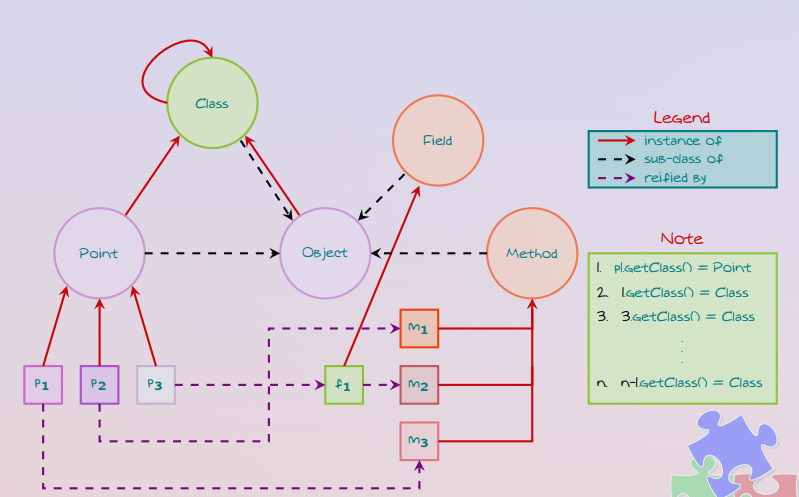
\includegraphics[scale=0.7]{8-the-javas-class-model}
\end{center}

\subsubsection{Java's Limitations on Reflaction}

\textbf{The meta-object protocol is no causally connected}
	- Causal connectionposes a security rick, which has not been analyzed in the context of Java's bytecode verifier

\textbf{Class is declared final}
	- One cannot create new meta-classes

\textbf{There are no MOP operations to modify classes)}
	- Therefore, one cannot easily create and modularize class-to-class transformation

\textbf{Do the Java designers disagree with such transformtations? No}

\subsection{Java Reflection API (Package java.lang.reflect)}

\subsubsection{Class-to-Class Transformations: Marker Interfaces}

\textbf{Consider}
\begin{itemize}
	\item Clonable
	\item Remote
	\item Serializable
\end{itemize}

Are these really interfaces? No

If not, what are they?
	- built-in class-to-class transformations

Java programmers cannot directly create such transformations

Other techniques must be employed ...
	- Some of them are the subject of the rest of this course

\subsubsection{Methods of Object}

\textbf{Object defines method to which all objects respond}

\begin{lstlisting}[language=Java]
class Object {
	public final Class<?> getClass() { ... }
	protected Object clone() { ... }
	public boolean equals(Object obj) { ... }
	public int hashcode() { ... }
	public String toString() { ... }
	public final void notify() { ... }
	public final void notifyAll() { ... }
	public final void wait() { ... }
		...
}
\end{lstlisting}

\subsubsection{Methods of Class<T>}

\textbf{Methods of Class<T>—Basic Operations}

\begin{lstlisting}[language=Java]
public final class Class<T> extends Object {
	public static Class<?> forName(String className) { ... }
	public static Class<?> forName(Module module, String name) { ... }
	public T newInstance() { ... } /* deprecated since 9 */
	public boolean isInstance(Object obj) { ... }
	public String getName() { ... }
	public Class<? super T> getSuperclass() { ... }
	public Module getModule() { ... }
	public Class<?>[] getInterfaces() { ... }
	public Class<?>[] getDeclaredClasses() throws SecurityException { ... }
	public Method[] getDeclaredMethods() throws SecurityException { ... }
	public Constructor<?> getEnclosingConstructor()
			throws SecurityException { ... }
	public Field[] getFields() throws SecurityException { ... }
		...
}
\end{lstlisting}

\subsubsection{java.lang.Class at Work}

\textbf{Let's write a method to return a printable class name}

\begin{lstlisting}[language=Java]
class MOP {
	public static String classNameToString(Class<?> cls) {
		if (!cls.isArray()) return cls.getName();
		else return cls.getComponentType().getName() + "[]";
	}
}
\end{lstlisting}

\begin{lstlisting}[language=Java]
[14:40]cazzola@hymir:~/tsp>jshell
| Welcome to JShell -- Version 11
| For an introduction type: /help intro
jshell> /open MOP1.java
jshell> MOP.classNameToString(String.class)
$2 ==> "java.lang.String"
jshell> var a = new Integer[]{1,2,3}
a ==> Integer[3] { 1, 2, 3 }
jshell> a.getClass()
$4 ==> class [Ljava.lang.Integer;
jshell> MOP.classNameToString(a.getClass())
$5 ==> "java.lang.Integer[]"
jshell> /exit
| Goodbye
\end{lstlisting}

\textbf{Let’s code a method to return super class hierarchy of a class}

\begin{lstlisting}[language=Java]
import java.util.ArrayList;
import java.util.List;

class MOP {
	public static Class<?>[] getAllSuperClasses(Class<?> cls) {
		List<Class<?>> result = new ArrayList<Class<?>>();
		for (Class<?> x = cls; x != null; x = x.getSuperclass())
			result.add(x) ;
		return result.toArray(new Class<?>[0]);
	}
}
\end{lstlisting}

\begin{lstlisting}[language=Java]
[16:33]cazzola@hymir:~/tsp>jshell
jshell> /open MOP2.java
jshell> MOP.getAllSuperClasses(java.util.ArrayList.class)
$4 ==> Class[4] { class java.util.ArrayList, class java.util.AbstractList,
                  class java.util.AbstractCollection, class java.lang.Object }
\end{lstlisting}

\subsubsection{Summary for Class<T> Methods}

\textbf{Member Access}

getAnnotations
getAnnotation
getClasses
getConstructors
getConstructor
getDeclaredAnnotation
getDeclaredClasses
getDeclaredConstructors
getDeclaredConstructor
getDeclaredFields
getDeclaredField
getDeclaredMethods
getDeclaredMethod
getFields
getField
getMethods
getMethod

\textbf{Class Properties}

getComponentType
getDeclaringClass
getEnclosingClass
getEnclosingConstructor
getEnclosingMethod
getModifiers
isAnnotationPresent
isAnnotation
isAnonymousClass
isArray
isAssignableFrom
isEnum
isInterface
isPrimitive

\textbf{Context Access}

getClassLoader
getInterfaces
getModule
getPackage
getProtectionDomain
getResourceAsStream
getResource
getSigners

\subsubsection{Classes in java.lang.reflect}

\begin{center}
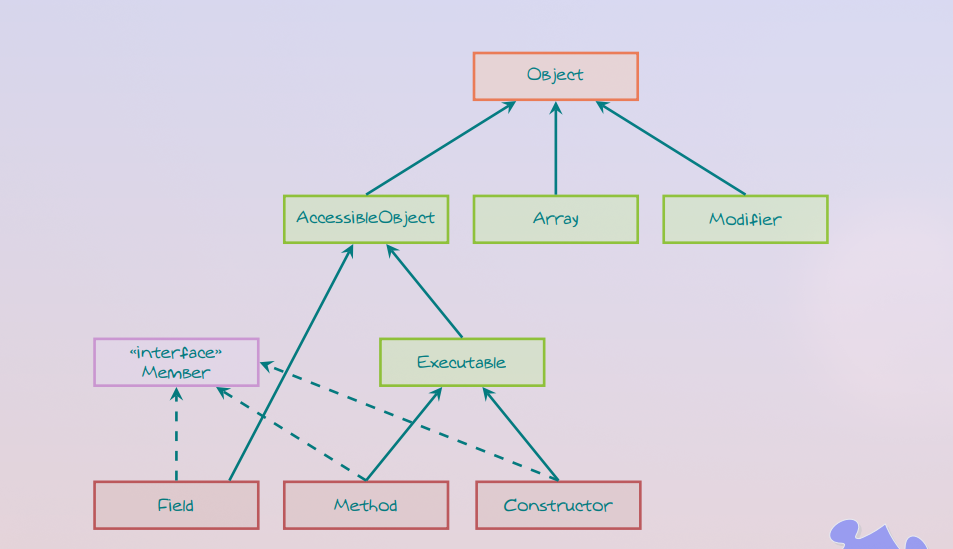
\includegraphics[scale=0.5]{9-classes-in-java-lang-reflected}
\end{center}

Instances of Field, Constructor, and Method are meta-objects

\subsubsection{java.lang.reflect.Method}

\begin{lstlisting}[language=Java]
public final class Method extends Executable implements Member {
	public Class<?> getReturnType() { ... }
	public Class<?>[] getParameterTypes() { ... }
	public Class<?>[] getExceptionTypes() { ... }
	public Object invoke(Object obj, Object... args)
		throws IllegalAccessException, IllegalArgumentException,
			InvocationTargetException { ... }
			...
}
\end{lstlisting}

\subsubsection{When using invoke:}

\begin{itemize}
	\item individual parameters are automatically unwrapped to match primitive formal parameters, and
	\item both primitive and reference parameters are subject to method
invocation conversions as necessary.
\end{itemize}

\textbf{The return type is automatically wrapped in an Object}

\begin{lstlisting}[language=Java]
import java.util.stream.*;
import java.util.Arrays;
import java.lang.reflect.Method;

class MOP {
	public static String headerSuffixToString(Method m) {
		String result = MOP.classNameToString( m.getReturnType() )
				+ " " + m.getName()
				+ "(" + MOP.formalParametersToString( m ) + ")";
		Class<?>[] exs = m.getExceptionTypes();
		if (exs.length > 0)
			result += " throws " + MOP.classArrayToString(exs);
		return result;
	}
}
\end{lstlisting}

\begin{lstlisting}[language=Java]
[20:28]cazzola@hymir:~/tsp>jshell
jshell> /open MOP4.java
jshell> var cls = Class.forName("java.lang.reflect.Method")
cls ==> class java.lang.reflect.Method
jshell> var ms = Arrays.asList(cls.getDeclaredMethods()).stream()
	.filter(s->s.getName()=="invoke")
ms ==> java.util.stream.ReferencePipeline$2@548e7350
jshell> ms.forEach(m -> System.out.println(MOP.headerSuffixToString(m)))
java.lang.Object invoke(java.lang.Object p1, java.lang.Object[] p2)
	throws java.lang.IllegalAccessException,
			java.lang.IllegalArgumentException,
	java.lang.reflect.InvocationTargetException
\end{lstlisting}

\subsubsection{java.lang.reflect.Field}

\begin{lstlisting}[language=Java]
public final class Field extends AccessibleObject implements Member {
	public Class<?> getType() { ... };
	public Object get(Object obj)
		throws IllegalArgumentException, IllegalAccessException { ... };
	public void set(Object obj, Object value)
		throws IllegalArgumentException, IllegalAccessException { ... };
	public Class<?> getDeclaringClass() {...} ;
		... // Include get* and set* for the eight primitive types
}
\end{lstlisting}

\subsubsection{java.lang.reflect.AccessibleObject}

\textbf{Purpose}
It is the base class for Field, Method and Constructor objects
	- In this last two cases inherited by the Executable class.

It enables the suppression of the access control checks when:
\begin{itemize}
	\item setting or getting fields (using Field)
	\item invoking methods (using Method)
	\item  creating and initializing new instances of classes (Constructor)
\end{itemize}

\begin{lstlisting}[language=Java]
public final class AccessibleObject {
	public void setAccessible(boolean flag) throws SecurityException { ... }
	public static void setAccessible(AccessibleObject[] array, boolean flag)
			throws SecurityException { ... }
	public boolean isAccessible() { ... }
}
\end{lstlisting}

\textbf{Note that the Java security manager can forbid the use of setAccessible()}

\subsubsection{java.lang.reflect.AccessibleObject (Cont'd)}

\begin{lstlisting}[language=Java]
import java.lang.reflect.Field;

class Employee {
	private String name;
	public Employee(String name) { this.name = name; }
}

class AccessibilityCheck {
	public static void main(String[] args) {
		try {
			Employee mike = new Employee("Mike");
			Field name = Employee.class.getDeclaredField("name");
			name.setAccessible(true);
			System.out.println("Value of name: "+ name.get(mike));
			name.set(mike, "Eleonor");
			System.out.println("Changed value of name: " + name.get(mike));
		} catch(NoSuchFieldException | SecurityException |
				IllegalAccessException e) {
			System.out.println(e.getMessage());
		}
	}
}
\end{lstlisting}

\begin{lstlisting}[language=Java]
grant {
	permission java.lang.reflect.ReflectPermission
	"suppressAccessChecks";
};
\end{lstlisting}

\begin{lstlisting}[language=Java]
[22:53]cazzola@hymir:~/tsp>java AccessibilityCheck
Value of name: Mike
Changed value of name: Eleonor
[23:02]cazzola@hymir:~/tsp>java -Djava.security.manager AccessibilityCheck
access denied ("java.lang.reflect.ReflectPermission" "suppressAccessChecks")
[23:03]cazzola@hymir:~/tsp>java -Djava.security.policy=granted.policy
                                -Djava.security.manager AccessibilityCheck
Value of name: Mike
Changed value of name: Eleonor
\end{lstlisting}

\subsubsection{java.lang.reflect.Constructor}

\begin{lstlisting}[language=Java]
public final class Constructor extends AccessibleObject implements Member {
	public T newInstance(Object... initargs)
		throws InstantiationException, IllegalAccessException,
			IllegalArgumentException, InvocationTargetException { ... }
	...
}
\end{lstlisting}

\textbf{Note that newInstance() of Class invokes default constructor, other constructor are invoked with newInstance() of Constructor}

\subsubsection{Examples: Smart Reflective Access to Fields}

\begin{lstlisting}[language=Java]
import java.lang.reflect.*;

public interface SmartFieldAccess {
	default public Object instVarAt(String name) throws Exception {
		Field f = this.getClass().getDeclaredField(name);
		f.setAccessible(true);
		if (!Modifier.isStatic(f.getModifiers())) return f.get(this);
		return null;
}

default public void instVarAtPut(String name, Object value)
			throws Exception {
	Field f = this.getClass().getDeclaredField(name);
	f.setAccessible(true);
	if (!Modifier.isStatic(f.getModifiers())) f.set(this, value);
	}
}

class Employee implements SmartFieldAccess {
	private String name;
	public Employee(String name) {this.name=name;}
}
\end{lstlisting}

\begin{lstlisting}[language=Java]
[0:24]cazzola@hymir:~/tsp>jshell
jshell> /open SmartFieldAccess.java
jshell> var mike = new Employee("Mike");
mike ==> Employee@59f99ea
jshell> mike.instVarAtPut("name", "Eleonor")
jshell> mike.instVarAt("name")
$6 ==> "Eleonor"
\end{lstlisting}

\subsubsection{Examples: Reflective Cloning}

\begin{lstlisting}[language=Java]
import java.lang.reflect.Field;

public interface ReflectiveCloning {
	default public Object copy() throws Exception {
		Object tmp = this.getClass().getDeclaredConstructor()
						.newInstance() ;
		Field[] fields = this.getClass().getDeclaredFields();
		for (int i = 0; i < fields.length; i++) {
			fields[i].setAccessible(true);
			fields[i].set(tmp, fields[i].get(this));
		}
		return tmp;
	}
}

class Employee implements ReflectiveCloning {
	private String name;
	public Employee() {this.name="Anon"; }
	public Employee(String name) {this.name=name;}
	public String toString() {return "Employee: "+this.name;}
}
\end{lstlisting}

\begin{lstlisting}[language=Java]
[1:04]cazzola@hymir:~/tsp>jshell
jshell> /open ReflectiveCloning.java
jshell> var e = new Employee("Mike");
e ==> Employee: Mike
jshell> var e1 = e.copy();
e1 ==> Employee: Mike
\end{lstlisting}

\subsubsection{Examples: Reflective Cloning}

\begin{lstlisting}[language=Java]
import java.lang.reflect.Method;

public interface SmartMessageSending {
	default public Object receive(String selector, Object[] args)
				throws Exception {
		Method mth = null; Class<?>[] classes = null;
		if (args != null) {
			classes = new Class<?>[args.length];
			for (int i = 0; i < args.length; i++) classes[i] = args[i].getClass();
		}
		mth = this.getClass().getMethod(selector, classes);
		return mth.invoke(this, args);
	}
}

class Employee implements SmartMessageSending {
	private String name;
	public Employee(String name) {this.name=name;}
	public void setName(String name) {this.name=name;}
	public String getName() {return this.name;}
	public String toString() {return "Employee: "+this.name;}
}
\end{lstlisting}

\begin{lstlisting}[language=Java]
jshell> var e = new Employee("Mike");
e ==> Employee: Mike
jshell> e.receive("getName", null)
$1 ==> "Mike"
jshell> e.receive("setName", new Object[]{"Eleonor"})
$2 ==> null
jshell> e
e ==> Employee: Eleonor
\end{lstlisting}

\subsection{Conclusions}

\textbf{Benefits}
\begin{itemize}
	\item reflection in Java opens up the structure and the execution trace of the program
	\item the reflective API is simple and quite complete
\end{itemize}

\textbf{Drawbacks}
\begin{itemize}
	\item reflection in Java is limited to introspection
	\item there isn’t a clear separation between the two logical layers (baseand meta-level)
	\item reflection in Java has been proved inefficient
\end{itemize}
